\documentclass[aspectratio=169,9pt]{beamer}
\usetheme[
progressbar=frametitle,
progressbar=foot,
sectionpage=progressbar,
numbering=none,
]{metropolis}

\usepackage[spanish]{babel}
\usepackage[utf8]{inputenc}

%\usetheme[secheader]{Boadilla}

\usepackage{booktabs}
\usepackage{caption}
\usepackage{manyfoot}
\usepackage{lipsum}
\usepackage{makecell}
\usepackage{multirow}
\usepackage{soul}
\usepackage{xcolor}

% Azul
\definecolor{MainColor}{HTML}{004c8c}
\definecolor{Alert}{HTML}{0277bd}
\setbeamercolor{background canvas}{bg=white}
\setbeamercolor{frametitle}{bg=MainColor}
\setbeamercolor{alerted text}{fg=Alert}

%Magenta
\definecolor{Magenta}{rgb}{1.0, 0.0, 1.0}
%ForestGreen
\definecolor{ForestGreen}{RGB}{34,139,34}

\setbeamertemplate{footline}{% 
	\hfill% 
	\usebeamercolor[fg]{page number in head/foot}% 
	\usebeamerfont{page number in head/foot}% 
	\insertframenumber%
	%\,/\,\inserttotalframenumber
	\kern1em\vskip2pt% 
}

\newcommand\blfootnote[1]{%
	\begingroup
	\renewcommand\thefootnote{}\footnote{#1}%
	\addtocounter{footnote}{-1}%
	\endgroup
	
}
\makeatletter
\def\blfootnote{\gdef\@thefnmark{}\@footnotetext}
\makeatother

%


\title{Bere}
\date{Febrero 2021-II}
\author{Berenice&Ricardo Montalvo Lezama}
\institute{Instituto de Investigaciones en Matemáticas Aplicadas y en Sistemas}

\begin{document}
%\maketitle

% % % % % % % % % % % % % % % % % % % % % % % % % %
\begin{frame}
	\begin{center}
		\normalsize{UNIVERSIDAD NACIONAL AUTÓNOMA DE MÉXICO}\\
		\vspace{1mm}
		\normalsize{Licenciatura en Ciencia de Datos}\\
		\vspace{7mm}
		\Large{
			\color{MainColor}
			\href{http://turing.iimas.unam.mx/~bereml/course/iap/}
			{Introducción al Aprendizaje Profundo}
		}\\
		\vspace{2mm}
		\Large{Redes densas poco profundas}\\
		\vspace{7mm}
		\normalsize{Profesores:} \\
		\normalsize{Berenice \& Ricardo Montalvo Lezama} \\
		\medskip
		\footnotesize{Marzo 2021}
		\\\vspace{5mm}
		\normalsize{\href{http://turing.iimas.unam.mx/~gibranfp/cursos/aprendizaje_profundo/}{Contenido basado en el curso de AP del Dr. Gibran Fuentes Pineda del PCIC}} \\
	\end{center}
\end{frame}

% % % % % % % % % % % % % % % % % % % % % % % % % %
\begin{frame}{Regresión y clasificación}
	\begin{center}
		\includegraphics[scale=.78]{fig/reg_cls.pdf}
	\end{center}
\end{frame}


% % % % % % % % % % % % % % % % % % % % % % % % % %
\begin{frame}{Aprendizaje supervisado}
\begin{center}
	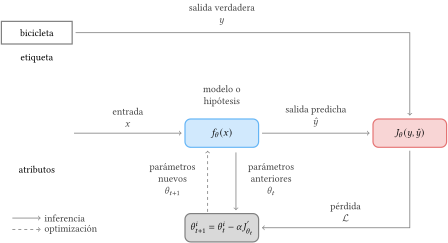
\includegraphics[scale=.8]{fig/supervisado.pdf}
\end{center}
\end{frame}

%
%% % % % % % % % % % % % % % % % % % % % % % % % % %
%\begin{frame}{Regresión lineal simple: hipótesis}
%	\begin{columns}
%		\begin{column}{0.55\textwidth}
%			\begin{flushleft}
%				\includegraphics[scale=.37]{fig/model_example.pdf}
%			\end{flushleft}
%		\end{column}
%		\begin{column}{0.45\textwidth}
%			
%			\begin{itemize}
%				\item Hipótesis:
%				\begin{equation*}
%					\hat{y}=  f(x;\theta) = x  w+b
%				\end{equation*}
%			\end{itemize}
%			
%		\end{column}
%	\end{columns}
%\end{frame}


% % % % % % % % % % % % % % % % % % % % % % % % % %
\begin{frame}{Regresión lineal simple: hipótesis}
\begin{columns}
	\begin{column}{0.55\textwidth}
		\begin{flushleft}
			\includegraphics[scale=.37]{fig/model_example.pdf}
		\end{flushleft}

			\includegraphics[scale=0.1]{fig/lin_reg.png}
	\end{column}
	\begin{column}{0.45\textwidth}

			\begin{itemize}
				\item Hipótesis:
				\begin{equation*}
					\hat{y}=  f_\theta(x) = x  w+b    \hspace{10mm} \theta = \{w,b\} 
				\end{equation*}
			\end{itemize}

	\end{column}
\end{columns}
\end{frame}

% % % % % % % % % % % % % % % % % % % % % % % % % %
\begin{frame}{Regresión lineal simple: pérdida}
	\begin{columns}
		\begin{column}{0.55\textwidth}
			\begin{flushleft}
				\includegraphics[scale=.5]{fig/error.pdf}
			\end{flushleft}
		\end{column}
		\begin{column}{0.45\textwidth}
				\begin{itemize}
					\item Hipótesis:
					\begin{equation*}
					\hat{y}=  f_\theta(x) = x  w+b    \hspace{10mm} \theta = \{w,b\} 
					\end{equation*}
					\item Función de error: error cuadrático medio 
					\begin{equation*}
						J_\theta = \frac{1}{2m}  \sum_{i=1}^{n}(y - \hat{y})^2
					\end{equation*}	
				\end{itemize}
		\end{column}
	\end{columns}
\end{frame}

% % % % % % % % % % % % % % % % % % % % % % % % % %
\begin{frame}{Descenso por gradiente}
	\begin{columns}
		\begin{column}{0.55\textwidth}
			\begin{flushleft}
				\includegraphics[scale=.5]{fig/cost_func.pdf}
			\end{flushleft}
		\end{column}
		\begin{column}{0.45\textwidth}
			\texttt{Repetir hasta converger:}\\ 
			\begin{center}
				\begin{equation*}
					\theta_{t+1}=\theta_{t}-\alpha \nabla J_{\theta_{t}}
				\end{equation*}
			\end{center}
		\end{column}
	\end{columns}
\end{frame}


% % % % % % % % % % % % % % % % % % % % % % % % % %
\begin{frame}{Descenso por gradiente para regresión lineal}
	\begin{columns}
		\begin{column}{0.55\textwidth}
			\begin{flushleft}
				\includegraphics[scale=.5]{fig/cost_func.pdf}
			\end{flushleft}
		\end{column}
		\begin{column}{0.45\textwidth}
			\texttt{Repetir hasta converger:} \vspace{-6mm}
			\begin{center}
			\begin{equation*}
				w := w  - \alpha \frac{\partial}{\partial w} J_\theta
			\end{equation*}		
			\begin{equation*}
				b := b  - \alpha \frac{\partial}{\partial b} J_\theta
			\end{equation*}
			\end{center}
			 \vspace{8mm}
			Cálculo de la derivadas:
			\begin{equation*}
			\frac{\partial}{\partial w} J_\theta  = \frac{1}{m} \sum_{i=1}^n (\hat{y}^{(i)} - y^{(i)}) \cdot x_j^{(i)}
			\end{equation*}
			\begin{equation*}
			 \frac{\partial}{\partial b} J_\theta = \frac{1}{m} \sum_{i=1}^n (\hat{y}^{(i)} - y^{(i)})
			\end{equation*}
		\end{column}
	\end{columns}
\end{frame}



% % % % % % % % % % % % % % % % % % % % % % % % % %
\begin{frame}{Hiperparámetro: tasa de aprendizaje}
	\begin{itemize}
		\item Tasa de aprendizaje muy grande.
	\end{itemize}
	\begin{center}
		\includegraphics[scale=2]{fig/tasa_grande.pdf}
	\end{center}
\end{frame}

% % % % % % % % % % % % % % % % % % % % % % % % % %
\begin{frame}{Hiperparámetro: tasa de aprendizaje}
	\begin{itemize}
		\item Tasa de aprendizaje muy pequeña.
	\end{itemize}
	\begin{center}
		\includegraphics[scale=2]{fig/tasa_chica.pdf}
	\end{center}
\end{frame}

% % % % % % % % % % % % % % % % % % % % % % % % % %
\begin{frame}{Hiperparámetro: tasa de aprendizaje}
	\begin{itemize}
		\item Tasa de aprendizaje adecuada.
	\end{itemize}
	\begin{center}
		\includegraphics[scale=2]{fig/tasa_adecuada.pdf}
	\end{center}
\end{frame}



% % % % % % % % % % % % % % % % % % % % % % % % % %

\begin{frame}{Sensibilidad a tasa de aprendizaje $\alpha$}
	\begin{center}
		\includegraphics[scale=0.7]{fig/gd_alfas.pdf}
	\end{center}
\end{frame}

% % % % % % % % % % % % % % % % % % % % % % % % % %
\begin{frame}{Ejemplo I del descenso por gradiente para regresión lineal}	
\begin{itemize}
	\item Inicializando $w_1$ con un valor mayor al que minimiza la función de pérdida 
\end{itemize}	
	\begin{center}
	\includegraphics[scale=.46]{fig/gd_init010it1.pdf}
	\end{center}
\end{frame}


% % % % % % % % % % % % % % % % % % % % % % % % % %
\begin{frame}{Ejemplo I del descenso por gradiente para regresión lineal}
\begin{itemize}
	\item Inicializando $w_1$ con un valor menor al que minimiza la función de pérdida
\end{itemize}	
	\begin{center}
		\includegraphics[scale=.46]{fig/gd_init010it2.pdf}
	\end{center}
\end{frame}

% % % % % % % % % % % % % % % % % % % % % % % % % %
\begin{frame}{Ejemplo I del descenso por gradiente para regresión lineal}
\begin{itemize}
	\item Inicializando $w_1$ con un valor menor al que minimiza la función de pérdida
\end{itemize}	
	\begin{center}
		\includegraphics[scale=.46]{fig/gd_init010it3.pdf}
	\end{center}
\end{frame}

% % % % % % % % % % % % % % % % % % % % % % % % % %
\begin{frame}{Ejemplo I del descenso por gradiente para regresión lineal}
\begin{itemize}
	\item Inicializando $w_1$ con un valor menor al que minimiza la función de pérdida
\end{itemize}	
	\begin{center}
		\includegraphics[scale=.46]{fig/gd_init010it8.pdf}
	\end{center}
\end{frame}

% % % % % % % % % % % % % % % % % % % % % % % % % %
\begin{frame}{Ejemplo II del descenso por gradiente para regresión lineal}
\begin{itemize}
	\item Inicializando $w_1$ con un valor mayor al que minimiza la función de pérdida
\end{itemize}
\begin{center}
	\includegraphics[scale=0.46]{fig/gd_init970it1.pdf}
\end{center}
\end{frame}

% % % % % % % % % % % % % % % % % % % % % % % % % %
\begin{frame}{Ejemplo II del descenso por gradiente para regresión lineal}
\begin{itemize}
	\item Inicializando $w_1$ con un valor mayor al que minimiza la función de pérdida
\end{itemize}
\begin{center}
	\includegraphics[scale=0.46]{fig/gd_init970it2.pdf}
\end{center}
\end{frame}

% % % % % % % % % % % % % % % % % % % % % % % % % %
\begin{frame}{Ejemplo II del descenso por gradiente para regresión lineal}
\begin{itemize}
	\item Inicializando $w_1$ con un valor mayor al que minimiza la función de pérdida
\end{itemize}
\begin{center}
	\includegraphics[scale=0.46]{fig/gd_init970it4.pdf}
\end{center}
\end{frame}


% % % % % % % % % % % % % % % % % % % % % % % % % %
\begin{frame}{Ejemplo II del descenso por gradiente para regresión lineal}
\begin{itemize}
	\item Inicializando $w_1$ con un valor mayor al que minimiza la función de pérdida
\end{itemize}
\begin{center}
	\includegraphics[scale=0.46]{fig/gd_init970it8.pdf}
\end{center}
\end{frame}





% % % % % % % % % % % % % % % % % % % % % % % % % %
%\begin{frame}{Regresión logística: hipótesis}
%	\begin{columns}
%		\begin{column}{0.55\textwidth}
%			\begin{flushleft}
%				\includegraphics[scale=.37]{fig/regresion_logistica.png}
%			\end{flushleft}
%		\end{column}
%		\begin{column}{0.45\textwidth}
%				\begin{itemize}
%					\item Hipótesis:
%					\begin{equation*}
%						P(y|x_i,\theta) = \hat{y}= \sigma(xw + b) =\frac{1}{1 + e^{-(xw + b)}}
%					\end{equation*}
%				\end{itemize}
%		\end{column}
%	\end{columns}
%\end{frame}

% % % % % % % % % % % % % % % % % % % % % % % % % %
\begin{frame}{Regresión logística: hipótesis}
	\begin{columns}
		\begin{column}{0.55\textwidth}
			\begin{flushleft}
				\includegraphics[scale=.33]{fig/regresion_logistica.png}
			\end{flushleft}
		\includegraphics[scale=.1]{fig/reg_log.png}
		\end{column}
		\begin{column}{0.55\textwidth}
			\begin{itemize}
				\item Hipótesis:
				\begin{equation*}
					P(y|x_i,\theta) = \hat{y}= \sigma(xw + b) =\frac{1}{1 + e^{-(xw + b)}}
				\end{equation*}
			\end{itemize}
		\end{column}
	\end{columns}
\end{frame}

% % % % % % % % % % % % % % % % % % % % % % % % % %
\begin{frame}{Regresión logística: pérdida}
	\begin{columns}
		\begin{column}{0.55\textwidth}
	\begin{flushleft}
		\includegraphics[scale=.33]{fig/regresion_logistica.png}
	\end{flushleft}
	\includegraphics[scale=.1]{fig/reg_log.png}
		\end{column}
		\begin{column}{0.55\textwidth}
			\begin{itemize}
				\item Hipótesis:
				\begin{equation*}
					P(y|x_i,\theta) = \hat{y}= \sigma(xw + b) =\frac{1}{1 + e^{-(xw + b)}}
				\end{equation*}
			
				\item Función de error: entropía cruzada binaria.
				\begin{equation*}
					J_\theta = - \frac{1}{m} \sum_{i=1}^{m} (y \log(\hat{y})+(1-y)log(1-\hat{y})) 
				\end{equation*}
			\end{itemize}
		\end{column}
	\end{columns}
\end{frame}

% % % % % % % % % % % % % % % % % % % % % % % % % %
\begin{frame}{Pérdida: entropía cruzada binaria}
	\begin{equation*}
		{J_\theta} = {\color{Magenta} (y)(-\log(\hat{y})) } + {\color{ForestGreen} (1-y)(-log(1-\hat{y})) }
	\end{equation*}
	\begin{columns}
		\begin{column}{0.7\textwidth}
			{\small
				\begin{table}[H]\centering
					\begin{tabular}{ccccc}
						\toprule
						\multirow{2}[3]*{} \makecell{Etiqueta\\$y$} &\makecell{Predicción\\ $\hat{y}$} &\makecell{Entropía\\binaria } & {Pérdida} & 
						\\
						\midrule
						{\color{ForestGreen}0}  & 	{\color{ForestGreen}0.9} &	{\color{ForestGreen} 2.303} & 	{\color{ForestGreen}alta } & \\
						{\color{ForestGreen}0}  & {\color{ForestGreen}0.1} & {\color{ForestGreen}0.105} & {\color{ForestGreen}baja}  & \\
						{\color{Magenta}1}  & {\color{Magenta}0.9} & {\color{Magenta}0.105} & {\color{Magenta}baja} & \\
						{\color{Magenta}1}  & {\color{Magenta}0.1} & {\color{Magenta}2.303} & {\color{Magenta}alta}  & \\
						\bottomrule
					\end{tabular}
				\end{table}
			}
		\end{column}
		\begin{column}{0.3\textwidth}
			\begin{flushleft}
				\includegraphics[scale=.23]{fig/log.png}
			\end{flushleft}
		\end{column}
	\end{columns}
\end{frame}
%
%% % % % % % % % % % % % % % % % % % % % % % % % % %
%\begin{frame}{Regresión logística: optimización}
%	\begin{columns}
%		\begin{column}{0.55\textwidth}
%	\begin{flushleft}
%		\includegraphics[scale=.33]{fig/regresion_logistica.png}
%	\end{flushleft}
%	\includegraphics[scale=.1]{fig/reg_log.png}
%		\end{column}
%		\begin{column}{0.55\textwidth}
%			\begin{itemize}
%				\item Modelo:
%				\begin{equation*}
%					P(y|x_i,\theta) = \hat{y}= \sigma(xw + b) =\frac{1}{1 + e^{-(xw + b)}}
%				\end{equation*}
%				\item Función de error: entropía cruzada binaria.
%				\begin{equation*}
%					\mathcal{L}(\theta) = - \frac{1}{m} \sum_{i=1}^{m} (y \log(\hat{y})+(1-y)log(1-\hat{y})) 
%				\end{equation*}
%				\item Optimización de la función de error:
%				\begin{equation*}
%					w := w  - \alpha \frac{\partial}{\partial w} \mathcal{L}(w, b)
%				\end{equation*}		
%				\begin{equation*}
%					b := b  - \alpha \frac{\partial}{\partial b}  \mathcal{L}(w, b)
%				\end{equation*}
%			\end{itemize}
%		\end{column}
%	\end{columns}
%\end{frame}

% % % % % % % % % % % % % % % % % % % % % % % % % %
\begin{frame}{Descenso por gradiente para regresión logística}

	\texttt{Repetir hasta converger:} \vspace{-6mm}
	\begin{center}
				\begin{equation*}
					w := w  - \alpha \frac{\partial}{\partial w} J_\theta
				\end{equation*}		
				\begin{equation*}
					b := b  - \alpha \frac{\partial}{\partial b}  J_\theta
				\end{equation*}
			\end{center}
			\vspace{8mm}
			Cálculo de la derivadas:
			\begin{equation*}
				\frac{\partial}{\partial w} J_\theta  = \frac{1}{n} \sum_{i=1}^n (\hat{y}^{(i)} - y^{(i)}) \cdot x_j^{(i)}
			\end{equation*}
			\begin{equation*}
				\frac{\partial}{\partial b}  J_\theta = \frac{1}{n} \sum_{i=1}^n (\hat{y}^{(i)} - y^{(i)})
			\end{equation*}
\end{frame}

% % % % % % % % % % % % % % % % % % % % % % % % % %
\begin{frame}{Regresión logística: métrica}
	\begin{columns}
		\begin{column}{0.55\textwidth}
		\begin{flushleft}
		\includegraphics[scale=.33]{fig/regresion_logistica.png}
		\end{flushleft}
		\includegraphics[scale=.1]{fig/reg_log.png}
		\end{column}
		\begin{column}{0.55\textwidth}
			\begin{itemize}
				\item Modelo:
				\begin{equation*}
				P(y|x_i,\theta) = \hat{y}= \sigma(xw + b) =\frac{1}{1 + e^{-(xw + b)}}
				\end{equation*}
				\item Función de error: entropía cruzada binaria.
				\begin{equation*}	
					J_\theta = - \frac{1}{m} \sum_{i=1}^{m} (y \log(\hat{y})+(1-y)log(1-\hat{y})) 
				\end{equation*}
				\item Optimización de la función de error:
				\begin{equation*}
					w := w  - \alpha \frac{\partial}{\partial w} J_\theta
				\end{equation*}		
				\begin{equation*}
					b := b  - \alpha \frac{\partial}{\partial b} J_\theta
				\end{equation*}
				\item Métrica: exactitud. 
				\begin{equation*}
					Ex = \frac{\text{ $\#$ predicciones correctas}}{\text{$\#$ total de predicciones}}
				\end{equation*}					
			\end{itemize}
			
		\end{column}
	\end{columns}
\end{frame}

% % % % % % % % % % % % % % % % % % % % % % % % % %
\begin{frame}{Partición de datos}
	\begin{center}
		\includegraphics[scale=1]{fig/dataset_partition.pdf}
	\end{center}
\end{frame}


% % % % % % % % % % % % % % % % % % % % % % % % % %
\begin{frame}{Clasificación multietiqueta}
 \begin{center}
	\includegraphics[scale=0.25]{fig/multi_logreg.pdf}
\end{center}

\begin{itemize}
	\item Función de pérdida: entropía cruzada binaria de cada categoría
	$$
		J_\theta({y}_k, \mathbf{\hat{y}}_k) = -\sum_{i=1}^N  \left[ y^{(i)}_k \log{\hat{y}^{(i)}_k} + (1 - y^{(i)}_k) \log{(1 - \hat{y}^{(i)}_k)} \right]
	$$
\end{itemize}
\end{frame}


% % % % % % % % % % % % % % % % % % % % % % % % % %
\begin{frame}{Clasificación multiclase}
\begin{columns}
	\begin{column}{0.50\textwidth}
		\begin{itemize}
			\item Neuronas de la capa de salida tienen una función de activación $softmax$ compartida, dada por
			$$
			softmax(\mathbf{z})_i = \frac{e^{z_i}}{\sum_{j = 1}^K e^{z_j}}, i = 1, \ldots, K
			$$
		\end{itemize}
	\end{column}
	\begin{column}{0.40\textwidth}
			\begin{center}
			\includegraphics[scale=0.3]{fig/softmax.pdf}
		\end{center}
	\end{column}
\end{columns}
\end{frame}


%% % % % % % % % % % % % % % % % % % % % % % % % % %
%\begin{frame}{Clasificación Softmax (I)}
%\begin{center}
%	\includegraphics[scale=0.3]{fig/softmax.pdf}
%\end{center}
%\end{frame}
%
%% % % % % % % % % % % % % % % % % % % % % % % % % %
%\begin{frame}{Clasificación Softmax (II)}
%  \begin{itemize}
%	\item Neuronas de la capa de salida tienen una función de activación $softmax$ compartida, dada por
%	$$
%	softmax(\mathbf{z})_i = \frac{e^{z_i}}{\sum_{j = 1}^K e^{z_j}}, i = 1, \ldots, K
%	$$
%	\bigskip
%	\item Función de pérdida: entropía cruzada categórica
%	\begin{align*}
%		J_\theta(\mathbf{Y}, \mathbf{\hat{Y}}) & = -\sum_{i=1}^N\sum_{k=1}^K \left[y^{(i)}_k\cdot \log \frac{e^{z_k^{(i)}}}{\sum_j e^{z_j^{(i)}}}\right]
%		x_j^{(i)}\\
%		\frac{\partial J_\theta}{\partial w_j} & = \frac{1}{N} \sum_{i=1}^N (\mathbf{\hat{y}}^{(i)} - \mathbf{y}^{(i)}) \otimes	 \mathbf{x}^{(i)}\\
%		\frac{\partial J_\theta}{\partial b} & = \frac{1}{N} \sum_{i=1}^N (\mathbf{\hat{y}}^{(i)} - \mathbf{y}^{(i)})
%	\end{align*}	
%\end{itemize}
%\end{frame}

% % % % % % % % % % % % % % % % % % % % % % % % % %


\end{document}

